\chapter{更新日志}


\begin{longtable}{|m{50pt}|m{100pt}|m{250pt}|}
%head
\multicolumn{3}{r}{}
\tabularnewline\hline
日期&更新内容&备注
\endhead
%endhead

%firsthead
\caption{更新日志}\\
\hline
日期&更新内容&备注
\endfirsthead
%endfirsthead

%foot
\multicolumn{3}{r}{}
\endfoot
%endfoot

%lastfoot
\endlastfoot
%endlastfoot
\hline
2017-08-14  & 航班订阅接口建议fid格式 & 出发地三字码+目的地三字母+年月日+航班号(例如SHABJS170814CA1836),不能超过20个字符\\
\hline
2017-08-14  & 前序航班接口参数  & 前序航班必须传入出发地和目的地机场三字母\\
\hline
2017-08-15 & 航班订阅接口fid格式& fid中不能包含下划线等特殊字符,只支持数字和字母,长度不超过20个字符\\
\hline
2017-09-06&前序航班查询&经停航班后程会返回相同航班\\
\hline
\end{longtable}


\chapter{签名算法}

所有请求在发送之前必须进行签名,否则服务器无法处理。


\section{请求编码}


\begin{compactitem}
\item \texttt{application/x-www-form-urlencoded} (推荐)

如果使用CURL提交请求需要进行设置。

\item \texttt{json}

\end{compactitem}

如果请求体使用JSON字符串,格式参考如下:

\begin{figure}[htbp]
\centering
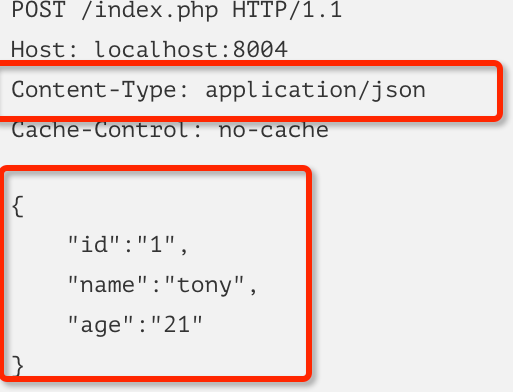
\includegraphics[scale=0.45]{post_json.png}
\caption{请求体使用JSON字符串}
\end{figure}


\section{签名示例}

对POST请求参数按照key的升序排序进行key=value拼接,并拼接上secret\_key后进行md5。

%\begin{lstlisting}[language=PHP]
%<?php
%$request = [
%   'api_key'=>'api_key_demo',
%   'date'=>'2017-10-15',
%   'departure'=>'SHA',
%   'arrival'=>'BJS'
%];
%ksort($request);
%$str = '';
%foreach ($request as $key=>$value) {
%  $str .= $key.'='.$value;
%}
%$str.=$secret_key;
%$secret_key = md5($str);
%\end{lstlisting}


\chapter{航班动态}


\section{接口地址}

/public/service/flight

\section{请求方法}


POST

\section{请求示例}

\texttt{POST /public/service/flight}


\section{请求参数}



\begin{longtable}{|m{60pt}|m{50pt}|m{80pt}|m{200pt}|}
%head
\multicolumn{4}{r}{}
\tabularnewline\hline
参数&是否可选&说明&备注
\endhead
%endhead

%firsthead
\caption{请求参数说明}\\
\hline
参数&是否可选&说明&备注
\endfirsthead
%endfirsthead

%foot
\multicolumn{4}{r}{}
\endfoot
%endfoot

%lastfoot
\endlastfoot
%endlastfoot
\hline
api\_key   & 必选 & apk\_key & 16位字符串\\
\hline
sign            &必选 & POST请求签名& 32位字符串\\
\hline
date	            &必选 & 行程日期         &YYYY-MM-DD\\
\hline
departure &可选 &	出发地三字码 &见请求参数说明\\
\hline
arrival        &可选 & 目的地三字码 &见请求参数说明\\
\hline
flight\_no &可选 & 航班号             &见请求参数说明\\
\hline
\end{longtable}

\begin{compactitem}
\item date:日期(格式YYYY-MM-DD)
\item departure:出发地三字代码(可以是城市代码或机场代码)
\item arrival:到达地三字代码(可以是城市代码或机场代码)
\item flight\_no:航班号
\end{compactitem}

\section{请求说明}

\begin{compactenum}
\item 传入date+departure+arrival返回航班动态列表(多个航班的动态)
\item 传入date+flight\_no返回航班动态详情(根据航班状态会返回多个数组)
\end{compactenum}

航班动态列表和航班动态详情使用同一个接口提供服务,根据传入的参数的不同返回不同的结果,但是结果格式是一致的。

\begin{compactitem}
\item 航班动态列表(传入出发代码/到达代码+日期)
\item 航班动态详情(传入航班号+日期)
\end{compactitem}

\section{返回代码说明}




\begin{longtable}{|m{30pt}|m{120pt}|m{200pt}|}
%head
\multicolumn{3}{r}{}
\tabularnewline\hline
代码&说明&备注
\endhead
%endhead

%firsthead
\caption{返回代码说明}\\
\hline
代码&说明&备注
\endfirsthead
%endfirsthead

%foot
\multicolumn{3}{r}{}
\endfoot
%endfoot

%lastfoot
\endlastfoot
%endlastfoot
\hline
200	&OK	                               &\\
\hline
400	&缺少日期                    &\\
\hline
400	&日期格式错误           &日期使用YYYY-MM-DD格式\\
\hline
400	&缺少出发/到达信息 &传入航班号或传入出发/到达\\
\hline
400	&无结果返回               &传入的请求参数实际上不存在\\
\hline
400	&缺少请求参数           &\\
\hline
400	&出发/到达代码有误&出发/到达代码都是大写的三字码(城市代码或机场代码)\\
\hline
400	&航班号格式错误      &\\
\hline
400	&网络请求异常           &\\
\hline
400	&网络请求失败          &\\
\hline
400	&解析数据失败          &\\
\hline
400	&返回数据为空         &\\
\hline
400	&接口请求失败         &\\
\hline
\end{longtable}


\section{返回参数说明}



\begin{longtable}{|m{100pt}|m{100pt}|m{180pt}|}
%head
\multicolumn{3}{r}{}
\tabularnewline\hline
参数&说明&备注
\endhead
%endhead

%firsthead
\caption{返回参数说明}\\
\hline
参数&说明&备注
\endfirsthead
%endfirsthead

%foot
\multicolumn{3}{r}{}
\endfoot
%endfoot

%lastfoot
\endlastfoot
%endlastfoot
\hline
FlightNo&航班号&\\
\hline
FlightCompany&航空公司名称&\\
\hline
FlightDepcode&出发地机场三字码&\\
\hline
FlightArrcode&目的地机场三字码&\\
\hline
FlightDeptimePlanDate&计划起飞时间&yyyy-mm-dd hh-mm-ss\\
\hline
FlightArrtimePlanDate&计划到达时间&yyyy-mm-dd hh-mm-ss\\
\hline
FlightDeptimeDate&实际起飞时间&yyyy-mm-dd hh-mm-ss\\
\hline
FlightArrtimeDate&实际到达时间&yyyy-mm-dd hh-mm-ss\\
\hline
stopFlag&是否经停&0:不经停;1:经停)\\
\hline
shareFlag&是否共享&0:不共享;1:共享)\\
\hline
VirtualFlag&是否虚拟&0:非虚拟航班;1:虚拟航班;未来航班返回为空\\
\hline
LegFlag&航段标识&0 计划航段;1 因备降而产生的航段;2 因返航而产生的航段\\
\hline
ShareFlightNo&共享航班号&实际承运航班的航班号\\
\hline
CheckinTable&值机柜台&\\
\hline
BoardGate&登机口&\\
\hline
BoardState&乘机状态&开始值机,值机结束,开始登机,催促登机,登机结束\\
\hline
FlightState&航班状态&计划、延误、取消、备降、返航、起飞、到达、备降起飞、备降取消、备降到达、返航起飞、返航取消、返航到达、提前取消\\
\hline
FlightDep&出发城市名&\\
\hline
FlightArr&到达城市名&\\
\hline
FlightDepAirport&出发机场名&\\
\hline
FlightArrAirport&到达机场名&\\
\hline
alternate\_info&备降信息节点&\\
\hline
AlternateStatus&备降后状态&\\
\hline
AlternateDepCity&备降后出发机场名&\\
\hline
AlternateArrCity&备降后到达机场名&\\
\hline
AlternateArrtimePlan&备降后计划到达时间&yyyy-mm-dd hh-mm-ss\\
\hline
AlternateDeptimePlan&备降后计划起飞时间&yyyy-mm-dd hh-mm-ss\\
\hline
AlternateArrtime&备降后实际到达时间&yyyy-mm-dd hh-mm-ss\\
\hline
AlternateDeptime&备降后实际起飞时间&yyyy-mm-dd hh-mm-ss\\
\hline
org\_timezone&出发地时区&\\
\hline
dst\_timezone&目的地时区&\\
\hline
fcategory&航班属性&0:国内-国内;1 国内-国际;2 国内-地区;3:地区-国际;4:国际-国际;5:未知\\
\hline
fid&&按航班标识符原值返回\\
\hline
FlightWaitData&飞机排队情况&\\
\hline
\end{longtable}

\section{返回参数示例}


\begin{lstlisting}[language=JavaScript]
{
  "code": 200,
  "msg": "请求成功",
  "data": [
    {
      "fcategory": "0",
      "FlightNo": "EU6678",
      "FlightCompany": "中国南方航空股份有限公司",
      "FlightDepcode": "PVG",
      "FlightArrcode": "CTU",
      "FlightDeptimePlanDate": "2017-08-06 20:00:00",
      "FlightArrtimePlanDate": "2017-08-06 00:00:00",
      "FlightDeptimeDate": "2017-08-06 20:20:00",
      "FlightArrtimeDate": "2017-08-06 23:58:00",
      "CheckinTable": "C28,D28,E28",
      "BoardGate": "B223",
      "BoardState": "正在登机",
      "FlightState": "备降",
      "org_timezone": "28800",
      "dst_timezone": "28800",
      "ShareFlightNo": "MU1234",
      "StopFlag": "0",
      "ShareFlag": "1",
      "VirtualFlag": "0",
      "LegFlag": "1",
      "FlightDep": "上海",
      "FlightArr": "成都",
      "FlightWaitData": "0",
      "FlightDepAirport": "上海浦东",
      "FlightArrAirport": "成都双流"
    }
  ]
}
\end{lstlisting}


\chapter{航班订阅}


\section{接口地址}

/public/service/feed

\section{请求方法}


POST

\section{请求示例}

\texttt{POST /public/service/feed}


\section{请求参数}



\begin{longtable}{|m{60pt}|m{50pt}|m{90pt}|m{180pt}|}
%head
\multicolumn{4}{r}{}
\tabularnewline\hline
参数&是否可选&说明&备注
\endhead
%endhead

%firsthead
\caption{请求参数说明}\\
\hline
参数&是否可选&说明&备注
\endfirsthead
%endfirsthead

%foot
\multicolumn{4}{r}{}
\endfoot
%endfoot

%lastfoot
\endlastfoot
%endlastfoot
\hline
api\_key   & 必选  & apk\_key & 16位字符串\\
\hline
sign            &必选  & POST请求签名&32位字符串\\
\hline
fid               & 必选 & 航班订阅标识符&出发地+目的地+年月日+航班号(例如SHABJS170814CA1836),不能超过20个字符\\
\hline
date	            &必选 & 行程日期         &YYYY-MM-DD\\
\hline
departure &必选 &	出发地机场三字码 &见请求参数说明\\
\hline
arrival        &必选 & 目的地机场三字码 &见请求参数说明\\
\hline
flight\_no &必选 & 航班号             &见请求参数说明\\
\hline
\end{longtable}

\begin{compactitem}
\item date:日期(格式YYYY-MM-DD)
\item departure:出发地三字代码(可以是城市代码或机场代码)
\item arrival:到达地三字代码(可以是城市代码或机场代码)
\item flight\_no:航班号
\end{compactitem}

\section{请求说明}

\begin{compactenum}
\item fid必须传入,不包含大写和特殊字符等
\item 出发地/目的地传入机场代码(硬性要求)
\end{compactenum}


\section{返回代码说明}




\begin{longtable}{|m{30pt}|m{120pt}|m{200pt}|}
%head
\multicolumn{3}{r}{}
\tabularnewline\hline
代码&说明&备注
\endhead
%endhead

%firsthead
\caption{返回代码说明}\\
\hline
代码&说明&备注
\endfirsthead
%endfirsthead

%foot
\multicolumn{3}{r}{}
\endfoot
%endfoot

%lastfoot
\endlastfoot
%endlastfoot
\hline
200	&OK	                               &\\
\hline
400	&缺少日期                    &\\
\hline
400	&日期格式错误           &日期使用YYYY-MM-DD格式\\
\hline
400  & 缺少航班号              &\\
\hline
400  & 航班号错误              &\\
\hline
400  & 航班号格式错误     &\\
\hline
400  &缺少航班号标识符  & fid必须传入\\
\hline
400  &航班号标识符格式有误& fid不能包含特殊字符\\
\hline
400 & 出发地/目的地机场代码错误& \\
\hline
400  & 出发地/目的地不存在 & \\
\hline
400	&缺少出发/到达信息 &传入航班号或传入出发/到达\\
\hline
400	&无结果返回               &传入的请求参数实际上不存在\\
\hline
400  & 订阅失败                  & \\
\hline
400	&网络请求异常           &\\
\hline
400	&网络请求失败          &\\
\hline
400	&解析数据失败          &\\
\hline
400	&返回数据为空         &\\
\hline
400	&接口请求失败         &\\
\hline
\end{longtable}


\section{返回参数说明}




\begin{longtable}{|m{100pt}|m{100pt}|m{180pt}|}
%head
\multicolumn{3}{r}{}
\tabularnewline\hline
参数&说明&备注
\endhead
%endhead

%firsthead
\caption{返回参数说明}\\
\hline
参数&说明&备注
\endfirsthead
%endfirsthead

%foot
\multicolumn{3}{r}{}
\endfoot
%endfoot

%lastfoot
\endlastfoot
%endlastfoot
\hline
FlightDeptimePlanDate & 计划起飞时间&yyyy-mm-dd hh-mm-ss 格式\\
\hline
FlightArrtimePlanDate  & 计划到达时间&yyyy-mm-dd hh-mm-ss 格式\\
\hline
\end{longtable}




\section{返回参数示例}

\begin{lstlisting}[language=JavaScript]
{
  "code": 200,
  "msg": "OK",
  "data": {
    "error_code": 8,
    "error": "定制成功",
    "FlightDeptimePlanDate": "2017-08-11 09:30:00",
    "FlightArrtimePlanDate": "2017-08-11 13:05:00"
  }
}
\end{lstlisting}


\chapter{前序航班}


\section{接口地址}

/public/service/preflight


\section{请求方法}

POST

\section{请求示例}

\texttt{POST /public/service/preflight}

\section{请求参数}



\begin{longtable}{|m{60pt}|m{50pt}|m{90pt}|m{160pt}|}
%head
\multicolumn{4}{r}{}
\tabularnewline\hline
参数&是否可选&说明&备注
\endhead
%endhead

%firsthead
\caption{请求参数说明}\\
\hline
参数&是否可选&说明&备注
\endfirsthead
%endfirsthead

%foot
\multicolumn{4}{r}{}
\endfoot
%endfoot

%lastfoot
\endlastfoot
%endlastfoot
\hline
api\_key   & 必选 & apk\_key & 16位字符串\\
\hline
sign            &必选 & POST请求签名& 32位字符串\\
\hline
date	            &必选 & 行程日期         &YYYY-MM-DD\\
\hline
departure &必选 &	出发地机场三字码 &必须是机场三字码\\
\hline
arrival        &必选 & 目的地机场三字码 &必须是机场三字母\\
\hline
flight\_no &必选 & 航班号             &见请求参数说明\\
\hline
\end{longtable}

\section{请求说明}

\begin{compactitem}
\item 需要按航班号 + 航段完全方式查询
\item 目前只提供查询当天航班的前序航班
\item 返回时间均为当地时间
\item 接口汉字返回的内容需要进行 URLDecode 解码
\end{compactitem}

\section{异常情况}

\begin{compactenum}
\item 如果使用经停航班的后程参数查询前序,会返回相同航班
\end{compactenum}


\section{返回代码说明}



\begin{longtable}{|m{30pt}|m{120pt}|m{200pt}|}
%head
\multicolumn{3}{r}{}
\tabularnewline\hline
代码&说明&备注
\endhead
%endhead

%firsthead
\caption{返回代码说明}\\
\hline
代码&说明&备注
\endfirsthead
%endfirsthead

%foot
\multicolumn{3}{r}{}
\endfoot
%endfoot

%lastfoot
\endlastfoot
%endlastfoot
\hline
200	&OK	                               &\\
\hline
400	&缺少日期                    &\\
\hline
400	&日期格式错误           &日期使用YYYY-MM-DD格式\\
\hline
400  & 缺少航班号              &\\
\hline
400  & 航班号错误              &\\
\hline
400  & 航班号格式错误     &\\
\hline
400 & 出发地/目的地机场代码错误& \\
\hline
400  & 出发地/目的地不存在 & \\
\hline
400	&缺少出发/到达信息 &传入航班号或传入出发/到达\\
\hline
400	&无结果返回               &传入的请求参数实际上不存在\\
\hline
400	&网络请求异常           &\\
\hline
400	&网络请求失败          &\\
\hline
400	&解析数据失败          &\\
\hline
400	&返回数据为空         &\\
\hline
400	&接口请求失败         &\\
\hline
\end{longtable}


\section{返回参数说明}

\begin{longtable}{|m{100pt}|m{100pt}|m{180pt}|}
%head
\multicolumn{3}{r}{}
\tabularnewline\hline
参数&说明&备注
\endhead
%endhead

%firsthead
\caption{返回参数说明}\\
\hline
参数&说明&备注
\endfirsthead
%endfirsthead

%foot
\multicolumn{3}{r}{}
\endfoot
%endfoot

%lastfoot
\endlastfoot
%endlastfoot
\hline
FlightState & 航班状态 & 见航班动态说明\\
\hline
FlightNo &航班号 & \\
\hline
org\_timezone &出发地时区&例如28800\\
\hline
dst\_timezone &目的地时区&例如28800\\
\hline
FlightDepcode &出发机场三字码\\
\hline
FlightArrcode &目的机场三字码&\\
\hline
\end{longtable}

\section{返回参数示例}



\begin{lstlisting}[language=JavaScript]
{
  "code": 200,
  "msg": "OK",
  "data": [
    {
      "FlightState": "计划",
      "FlightNo": "CA4394",
      "org_timezone": "28800",
      "dst_timezone": "28800",
      "FlightDepcode": "CAN",
      "FlightArrcode": "JZH",
      "FlightDeptimePlanDate": "2017-08-07 11:25",
      "FlightArrtimePlanDate": "2017-08-07 14:15",
      "FlightDeptimeDate": "2017-08-07 14:59",
      "FlightArrtimeDate": "",
      "FlightDep": "广州",
      "FlightDepAirport": "广州白云",
      "FlightArr": "九寨沟",
      "FlightArrAirport": "九寨沟黄龙"
    }
  ]
}
\end{lstlisting}







